% questions.tex —— 2018 年·全国Ⅰ卷·理科 · 题目内容片段（无答案）
% 由 tools/generate_projects.py 依来源总账自 2018/2018_数学真题_理_试题.md 生成，勿手改（改源 MD 后重跑）


\begin{gknotice}
\textbf{ 卷种提示}：本卷为文理分科时代的旧结构，含\textbf{现已取消}的选做题（第 22/23 题）与\textbf{已删除}的三视图考点（第 7 题）。适合\textbf{按知识点抽题}，不适合整套限时模拟。

\textbf{适用省份}：河南、河北、山西、江西、湖北、湖南、广东、安徽、福建、山东
\end{gknotice}

\par\medskip

\gkpart{一、选择题}

\begin{gktip}
本题共 12 小题，每小题 5 分，共 60 分。
\end{gktip}

\begin{question}
\gkti{1}设 $z=\dfrac{1-\mathrm i}{1+\mathrm i}+2\mathrm i$，则 $|z|=$（　　）

\begin{gkopts}(4)
\task A．$0$
\task B．$\dfrac12$
\task C．$1$
\task D．$\sqrt2$
\end{gkopts}

\end{question}
\begin{question}
\gkti{2}已知集合 $A=\left\{x\mid x^{2}-x-2>0\right\}$，则 $\complement_{\mathbf R}A=$（　　）

\begin{gkopts}(2)
\task A．$\{x\mid-1<x<2\}$
\task B．$\{x\mid-1\le x\le2\}$
\task C．$\{x\mid x<-1\}\cup\{x\mid x>2\}$
\task D．$\{x\mid x\le-1\}\cup\{x\mid x\ge2\}$
\end{gkopts}

\Needspace{0.5\textheight}
\end{question}
\begin{question}
\gkti{3}某地区经过一年的新农村建设，农村的经济收入增加了一倍，实现翻番。为更好地了解该地区农村的经济收入变化情况，统计了该地区新农村建设前后农村的经济收入构成比例，得到如下饼图：
\nopagebreak[4]
\begin{center}% 2018 全国Ⅰ卷 理3/文3：新农村建设前后经济收入构成比例（双饼图）
% 从 90° 起顺时针切分；标签放各扇区中线角上，小扇区标签外置并加引线
\begin{tikzpicture}[font=\footnotesize, scale=1.0]
  % ---------- 左：建设前（种植60 养殖30 三产6 其他4）----------
  \begin{scope}
    \draw (0,0) circle (1.7);
    \foreach \a in {90, -126, -234, -255.6} {\draw (0,0) -- (\a:1.7);}
    \node at (-18:0.95)  {\shortstack{种植收入\\ $60\%$}};
    \node at (-180:0.95) {\shortstack{养殖收入\\ $30\%$}};
    \draw (-244.8:1.6) -- (-244.8:2.0);
    \node at (-244.8:2.05) [above left, inner sep=1pt] {第三产业收入 $6\%$};
    \draw (-262.8:1.6) -- (-262.8:2.0);
    \node at (-262.8:2.05) [above right, inner sep=1pt] {其他收入 $4\%$};
    \node at (0,-2.15) {\small 建设前经济收入构成比例};
  \end{scope}
  % ---------- 右：建设后（种植37 养殖30 三产28 其他5）----------
  \begin{scope}[xshift=6.2cm]
    \draw (0,0) circle (1.7);
    \foreach \a in {90, -43.2, -151.2, -252} {\draw (0,0) -- (\a:1.7);}
    \node at (23.4:0.95)   {\shortstack{种植收入\\ $37\%$}};
    \node at (-97.2:0.95)  {\shortstack{养殖收入\\ $30\%$}};
    \node at (-201.6:0.92) {\shortstack{第三产业\\ 收入 $28\%$}};
    \draw (-261:1.6) -- (-261:2.0);
    \node at (-261:2.05) [above, inner sep=1.5pt] {其他收入 $5\%$};
    \node at (0,-2.15) {\small 建设后经济收入构成比例};
  \end{scope}
\end{tikzpicture}
\end{center}
\nopagebreak[4]
则下面结论中\textbf{不正确}的是（　　）

\begin{gkopts}(1)
\task A．新农村建设后，种植收入减少
\task B．新农村建设后，其他收入增加了一倍以上
\task C．新农村建设后，养殖收入增加了一倍
\task D．新农村建设后，养殖收入与第三产业收入的总和超过了经济收入的一半
\end{gkopts}

\end{question}
\begin{question}
\gkti{4}设 $S_n$ 为等差数列 $\left\{a_n\right\}$ 的前 $n$ 项和，若 $3S_3=S_2+S_4$，$a_1=2$，则 $a_5=$（　　）

\begin{gkopts}(4)
\task A．$-12$
\task B．$-10$
\task C．$10$
\task D．$12$
\end{gkopts}

\end{question}
\begin{question}
\gkti{5}设函数 $f(x)=x^{3}+(a-1)x^{2}+ax$。若 $f(x)$ 为奇函数，则曲线 $y=f(x)$ 在点 $(0,0)$ 处的切线方程为（　　）

\begin{gkopts}(4)
\task A．$y=-2x$
\task B．$y=-x$
\task C．$y=2x$
\task D．$y=x$
\end{gkopts}

\end{question}
\begin{question}
\gkti{6}在 $\triangle ABC$ 中，$AD$ 为 $BC$ 边上的中线，$E$ 为 $AD$ 的中点，则 $\overrightarrow{EB}=$（　　）

\begin{gkopts}(1)
\task A．$\dfrac34\overrightarrow{AB}-\dfrac14\overrightarrow{AC}$
\task B．$\dfrac14\overrightarrow{AB}-\dfrac34\overrightarrow{AC}$
\task C．$\dfrac34\overrightarrow{AB}+\dfrac14\overrightarrow{AC}$
\task D．$\dfrac14\overrightarrow{AB}+\dfrac34\overrightarrow{AC}$
\end{gkopts}

\Needspace{0.5\textheight}
\end{question}
\begin{question}
\gkti{7}某圆柱的高为 $2$，底面周长为 $16$，其三视图如图。圆柱表面上的点 $M$ 在正视图上的对应点为 $A$，圆柱表面上的点 $N$ 在左视图上的对应点为 $B$，则在此圆柱侧面上，从 $M$ 到 $N$ 的路径中，最短路径的长度为（　　）
\nopagebreak[4]
\begin{center}% 2018 全国Ⅰ卷 理7/文9：圆柱的三视图（正视图/左视图为矩形，俯视图为圆）
% M 在正视图上的对应点 A（左上角），N 在左视图上的对应点 B（右下角）
\begin{tikzpicture}[scale=0.62, font=\small]
  \draw (0,0) rectangle (4,1.6);
  \node[above left, inner sep=1pt] at (0,1.6) {$A$};
  \begin{scope}[xshift=5.2cm]
    \draw (0,0) rectangle (4,1.6);
    \node[below right, inner sep=1pt] at (4,0) {$B$};
  \end{scope}
  \begin{scope}[yshift=-3.1cm, xshift=2cm]
    \draw (0,0) circle (1.45);
  \end{scope}
\end{tikzpicture}
\end{center}
\nopagebreak[4]
\begin{gkopts}(4)
\task A．$2\sqrt{17}$
\task B．$2\sqrt5$
\task C．$3$
\task D．$2$
\end{gkopts}

\begin{gktip}
\textbf{注}：三视图在现行新课标中已删除。
\end{gktip}

\end{question}
\begin{question}
\gkti{8}设抛物线 $C:y^{2}=4x$ 的焦点为 $F$，过点 $(-2,0)$ 且斜率为 $\dfrac23$ 的直线与 $C$ 交于 $M$，$N$ 两点，则 $\overrightarrow{FM}\cdot\overrightarrow{FN}=$（　　）

\begin{gkopts}(4)
\task A．$5$
\task B．$6$
\task C．$7$
\task D．$8$
\end{gkopts}

\end{question}
\begin{question}
\gkti{9}已知函数 $f(x)=\begin{cases}\mathrm e^{x},&x\le0\\ \ln x,&x>0\end{cases}$，$g(x)=f(x)+x+a$。若 $g(x)$ 存在 $2$ 个零点，则 $a$ 的取值范围是（　　）

\begin{gkopts}(4)
\task A．$[-1,0)$
\task B．$[0,+\infty)$
\task C．$[-1,+\infty)$
\task D．$[1,+\infty)$
\end{gkopts}

\Needspace{0.5\textheight}
\end{question}
\begin{question}
\gkti{10}如图来自古希腊数学家希波克拉底所研究的几何图形。此图由三个半圆构成，三个半圆的直径分别为直角三角形 $ABC$ 的斜边 $BC$、直角边 $AB$、$AC$。$\triangle ABC$ 的三边所围成的区域记为 I，黑色部分记为 II，其余部分记为 III。在整个图形中随机取一点，此点取自 I，II，III 的概率分别记为 $p_1$，$p_2$，$p_3$，则（　　）
\nopagebreak[4]
\begin{center}% 2018 全国Ⅰ卷 理10：希波克拉底月牙
% 直角三角形 ABC（直角在 A），三个半圆直径分别为 BC、AB、AC
% 填充次序：先黑填两个小半圆，再白填大半圆（盖掉重叠弓形），最后斜纹填三角形
\begin{tikzpicture}[scale=0.9, font=\small]
  \coordinate (B) at (0,0);
  \coordinate (C) at (4,0);
  \coordinate (A) at (0.8,1.6);   % 在以 BC 为直径的圆上，∠BAC=90°
  % AB 为直径的半圆（外侧）：圆心 (0.4,0.8)，半径 √3.2/2
  \fill[black] (B) arc[start angle=243.435, delta angle=180, radius=0.894427];
  % AC 为直径的半圆（外侧）：圆心 (2.4,0.8)，半径 √12.8/2
  \fill[black] (A) arc[start angle=153.435, delta angle=180, radius=1.788854];
  % BC 为直径的大半圆（上侧）刷白
  \fill[white] (C) arc[start angle=0, delta angle=180, radius=2];
  % 三角形区域 I：斜线纹理
  \fill[pattern=north east lines] (A) -- (B) -- (C) -- cycle;
  % 描边
  \draw (A) -- (B) -- (C) -- cycle;
  \draw (B) arc[start angle=243.435, delta angle=180, radius=0.894427];
  \draw (A) arc[start angle=153.435, delta angle=180, radius=1.788854];
  \draw (C) arc[start angle=0, delta angle=180, radius=2];
  \node[above] at (A) {$A$};
  \node[below left] at (B) {$B$};
  \node[below right] at (C) {$C$};
\end{tikzpicture}
\end{center}
\nopagebreak[4]
\begin{gkopts}(4)
\task A．$p_1=p_2$
\task B．$p_1=p_3$
\task C．$p_2=p_3$
\task D．$p_1=p_2+p_3$
\end{gkopts}

\end{question}
\begin{question}
\gkti{11}已知双曲线 $C:\dfrac{x^{2}}3-y^{2}=1$，$O$ 为坐标原点，$F$ 为 $C$ 的右焦点，过 $F$ 的直线与 $C$ 的两条渐近线的交点分别为 $M$，$N$。若 $\triangle OMN$ 为直角三角形，则 $|MN|=$（　　）

\begin{gkopts}(4)
\task A．$\dfrac32$
\task B．$3$
\task C．$2\sqrt3$
\task D．$4$
\end{gkopts}

\end{question}
\begin{question}
\gkti{12}已知正方体的棱长为 $1$，每条棱所在直线与平面 $\alpha$ 所成的角相等，则 $\alpha$ 截此正方体所得截面面积的最大值为（　　）

\begin{gkopts}(2)
\task A．$\dfrac{3\sqrt3}4$
\task B．$\dfrac{2\sqrt3}3$
\task C．$\dfrac{3\sqrt2}4$
\task D．$\dfrac{\sqrt3}2$
\end{gkopts}

\par\medskip

\end{question}
\gkpart{二、填空题}

\begin{gktip}
本题共 4 小题，每小题 5 分，共 20 分。
\end{gktip}

\begin{question}
\gkti{13}若 $x$，$y$ 满足约束条件 $\begin{cases}x-2y-2\le0\\ x-y+1\ge0\\ y\le0\end{cases}$，则 $z=3x+2y$ 的最大值为 \gkblank{}．

\end{question}
\begin{question}
\gkti{14}记 $S_n$ 为数列 $\left\{a_n\right\}$ 的前 $n$ 项和，若 $S_n=2a_n+1$，则 $S_6=$ \gkblank{}．

\end{question}
\begin{question}
\gkti{15}从 $2$ 位女生、$4$ 位男生中选 $3$ 人参加科技比赛，且至少有 $1$ 位女生入选，则不同的选法共有 \gkblank{} 种。（用数字填写答案）

\end{question}
\begin{question}
\gkti{16}已知函数 $f(x)=2\sin x+\sin2x$，则 $f(x)$ 的最小值是 \gkblank{}．

\par\medskip

\end{question}
\gkpart{三、解答题}

\begin{gktip}
共 70 分。第 17～21 题为必考题，第 22、23 题为选考题。
\end{gktip}

\gksubpart{（一）必考题：共 60 分}

\begin{question}
\gkti{17}\textbf{（12 分）} 在平面四边形 $ABCD$ 中，$\angle ADC=90^\circ$，$\angle A=45^\circ$，$AB=2$，$BD=5$。

  (1) 求 $\cos\angle ADB$；

  (2) 若 $DC=2\sqrt2$，求 $BC$。

\Needspace{0.5\textheight}
\end{question}
\begin{question}
\gkti{18}\textbf{（12 分）} 如图，四边形 $ABCD$ 为正方形，$E$，$F$ 分别为 $AD$，$BC$ 的中点，以 $DF$ 为折痕把 $\triangle DFC$ 折起，使点 $C$ 到达点 $P$ 的位置，且 $PF\perp BF$。
\nopagebreak[4]
\begin{center}% 2018 全国Ⅰ卷 理18：正方形 ABCD 沿 DF 折起，C 到达 P（PF⊥BF）
% 底面为直角梯形 ABFD，E 为 AD 中点；虚线 C 为折叠前位置
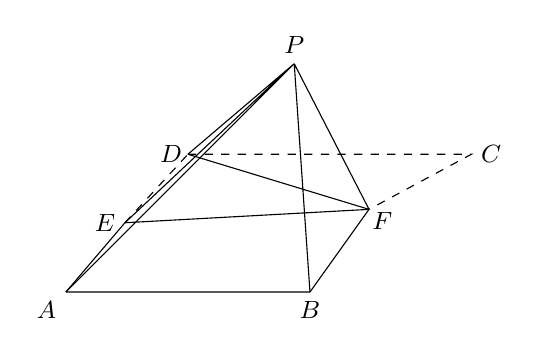
\begin{tikzpicture}[scale=1.0, font=\small]
  \coordinate (A) at (0,0);
  \coordinate (B) at (3.1,0);
  \coordinate (F) at (3.85,1.05);
  \coordinate (D) at (1.55,1.75);
  \coordinate (E) at (0.75,0.88);
  \coordinate (P) at (2.9,2.9);
  \coordinate (C) at (5.15,1.75);
  \draw (A) -- (B) -- (F);
  \draw (A) -- (E);
  \draw[dashed] (E) -- (D);
  \draw (D) -- (F);          % 折痕
  \draw (E) -- (F);
  \draw (A) -- (P)  (B) -- (P)  (F) -- (P)  (D) -- (P)  (E) -- (P);
  \draw[dashed] (D) -- (C) -- (F);
  \node[below left] at (A) {$A$};
  \node[below] at (B) {$B$};
  \node[below right, inner sep=1pt] at (F) {$F$};
  \node[left, inner sep=2pt] at (D) {$D$};
  \node[left] at (E) {$E$};
  \node[above] at (P) {$P$};
  \node[right] at (C) {$C$};
\end{tikzpicture}
\end{center}
\nopagebreak[4]
  (1) 证明：平面 $PEF\perp$ 平面 $ABFD$；

  (2) 求 $DP$ 与平面 $ABFD$ 所成角的正弦值。

\end{question}
\begin{question}
\gkti{19}\textbf{（12 分）} 设椭圆 $C:\dfrac{x^{2}}2+y^{2}=1$ 的右焦点为 $F$，过 $F$ 的直线 $l$ 与 $C$ 交于 $A$，$B$ 两点，点 $M$ 的坐标为 $(2,0)$。

  (1) 当 $l$ 与 $x$ 轴垂直时，求直线 $AM$ 的方程；

  (2) 设 $O$ 为坐标原点，证明：$\angle OMA=\angle OMB$。

\end{question}
\begin{question}
\gkti{20}\textbf{（12 分）} 某工厂的某种产品成箱包装，每箱 $200$ 件，每一箱产品在交付用户之前要对产品作检验，如检验出不合格品，则更换为合格品。检验时，先从这箱产品中任取 $20$ 件作检验，再根据检验结果决定是否对余下的所有产品作检验。设每件产品为不合格品的概率都为 $p\ (0<p<1)$，且各件产品是否为不合格品相互独立。

  (1) 记 $20$ 件产品中恰有 $2$ 件不合格品的概率为 $f(p)$，求 $f(p)$ 的最大值点 $p_0$；

  (2) 现对一箱产品检验了 $20$ 件，结果恰有 $2$ 件不合格品，以 (1) 中确定的 $p_0$ 作为 $p$ 的值。已知每件产品的检验费用为 $2$ 元，若有不合格品进入用户手中，则工厂要对每件不合格品支付 $25$ 元的赔偿费用。

  　① 若不对该箱余下的产品作检验，这一箱产品的检验费用与赔偿费用的和记为 $X$，求 $EX$；

  　② 以检验费用与赔偿费用和的期望值为决策依据，是否该对这箱余下的所有产品作检验？

\end{question}
\begin{question}
\gkti{21}\textbf{（12 分）} 已知函数 $f(x)=\dfrac1x-x+a\ln x$。

  (1) 讨论 $f(x)$ 的单调性；

  (2) 若 $f(x)$ 存在两个极值点 $x_1$，$x_2$，证明：$\dfrac{f\left(x_1\right)-f\left(x_2\right)}{x_1-x_2}<a-2$。

\par\medskip

\end{question}
\gksubpart{（二）选考题：共 10 分，第 22、23 题任选一题作答}

\begin{gktip}
\textbf{ 现行考纲已取消选做题}，以下两题仅作历史资料保留。
\end{gktip}

\begin{question}
\gkti{22}\textbf{（10 分）〔选修 4-4：坐标系与参数方程〕} （\textbf{已取消}）

在直角坐标系 $xOy$ 中，曲线 $C_1$ 的方程为 $y=k|x|+2$。以坐标原点为极点，$x$ 轴正半轴为极轴建立极坐标系，曲线 $C_2$ 的极坐标方程为 $\rho^{2}+2\rho\cos\theta-3=0$。

  (1) 求 $C_2$ 的直角坐标方程；

  (2) 若 $C_1$ 与 $C_2$ 有且仅有三个公共点，求 $C_1$ 的方程。

\end{question}
\begin{question}
\gkti{23}\textbf{（10 分）〔选修 4-5：不等式选讲〕} （\textbf{已取消}）

已知 $f(x)=|x+1|-|ax-1|$。

  (1) 当 $a=1$ 时，求不等式 $f(x)>1$ 的解集；

  (2) 若 $x\in(0,1)$ 时不等式 $f(x)>x$ 成立，求 $a$ 的取值范围。

\par\medskip


\end{question}